\label{subsec:cipt}
Now in the article \cite{cpt}, they also introduces the Coherent Interleaved Path
Tracing algorithm (also knwon as the CIPT algorithm), that in a coherency tile
is grouping pixels in a tile, according to a
latin hypercube. The idea of this implementation on the GPU is to assign set of
numbers to a given warp. But since a warp might have something like 32~threads,
we need a bigger latin hypercube. But not to big, because we want to keep the
cohenrency tile as small possible, to have closer raies as possible in a same
warp. But of course, the coherency tiles for the CIPT would be larger than for
the CPT, since we will have severals warps working on it.

Our implementation is using a lating hypercube using $4^2 = 16$ values. So the
coherency tile for the CIPT is a $16 \times 16$ pixels square. In order to assign
pixel position within the coherency tile for every threads of every warps
working on this tile, we are using a precomputed array that for a given $i$ and
position $y$, give the position $x$ with a $O(1)$ time complexity such as
$L_{y,x} = i$ with L is the latin hypercube's matrix notation.
\begin{figure}[H]
    \centering
    \begin{lstlisting}[morekeywords={uint32_t,uint32x2_t,get_global_id}]
// the thread id within the coherency tile
uint32_t threadId = get_global_id(0) % (16 * 16);

// the warp id within the coherency tile
uint32_t warpId = threadId / kWarpSize;

// the pixel position within the coherency tile
uint32x2_t pixelPos = (uint32x2_t)(
  latin_hypercube_x_pos(threadId / 16, threadId % 16),
  threadId % 16
);
    \end{lstlisting}
    \caption{CIPT's code assigning pixel position to each thread.}
    \label{code:cipt_pixel_pos}
\end{figure}

\begin{figure}[h]
    \centering
    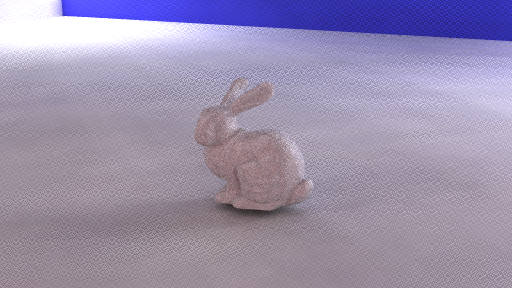
\includegraphics[width=0.8\columnwidth]{render_stanford_bunny.png}
    \caption{Stanford bunny rendered with a coherent interleaved path tracer algorithm.}
    \label{fig:stanford_bunny_cipt}
\end{figure}
This has the benefit to increase the number of distinct random seed values per
tile than the CPT algorithm, by introducing some noise. But note that you can
shufle the $x$ and $y$ position by reusing \textit{latin\_hypercube\_x\_pos()}
(Figure~\ref{code:cipt_pixel_pos}) for each sample of a same pixel, so that the latin
hypercube becomes less visible in the newly introduced noise. But compared to the
original article \cite{cpt}, the CIPT has a significant performance drop on GPU
of 30\% according to Figure~\ref{table:cipt_compare} compared to the CPT. That
is due to the warp efficency drop, caused by the fact that the parrallel raies computed in
the same warp are not as close as they are in the CPT algorithm, since the coherency
tile has to be larger, in order to have severals warps - with different random
seed values - working on it. But as the resolution is increasing, we can witness
experimetaly that this performance drop is becoming less important. In the end,
with a given warp size of $32$~threads (might depends on the wardware), we have only
a $30\%$ performance drop for $16^2 / 32 = 8$ times more samples with noise on a
tile as small as $4 \times 4$ pixels (thanks to the property of the latin hypercube),
and therefore less artefacts as we can see on Figure~\ref{fig:stanford_bunny_cipt}
compared to Figure~\ref{fig:stanford_bunny_cpt}.

\begin{figure}[H]
    \tiny
    \centering
    \begin{tabular}{ | l | c | c | }

        \hline
        Algorithm used & Bunny \\
        \hline
        Simple path tracer & 224.0ns \\
        Coherent interleaved path tracer & 134.6ns \\
        \hline

    \end{tabular}
    \caption{
        Per ray rendering time comparaison between a simple path tracer
        algorithm and a coherent interleaved path tracer (resolution of 512~x~288; 512
        sample per pixels; 9 recursive raies per samples).
    }
    \label{table:cipt_compare}
\end{figure}
